\chapter{Data fusion for virtual visualization}

\section{Introduction}

The previous two chapters developed two pipelines that can obtain broccoli head parts using close-range and aerial approaches. The aerial approach can obtain low-quality broccoli canopy models of the full field while the close-range approach can obtain high-quality broccoli head 3D models. As the next step, we targeted transforming and placing the high-quality head 3D models into the low-quality full field canopy models, targeted for 3D virtual visualization and explanation for a more intuitive feeling of growth status compare to numeric statistical values. It is also a fundamental and critical technique for virtual farmland and digital twin \citep{pylianidis_introducing_2021, slob_virtual_2023}. Until now, to the best of our knowledge, no published research has addressed this problem in the actual broccoli farmland. However, there are also several challenges to be solved before achieving that point. 

% what is backward project , what is forward projection
The first challenge is a more precise geographical location. Due to the low quality of the aerial model, in Chapter 3, we segmented the broccoli head on the raw images without geo-coordinate. However, during the backward projection from 3D geographical coordinates (3D canopy model) to the 2D pixel coordinate (2D raw image), one dimension is lost and not reversible. So, when forward projecting the broccoli head segmentation 2D coordinates back to the 3D geographical coordinate; for each vertex (point) of broccoli head polygons, instead of getting precise 3D geographical points, only a ray ($Z_{cam}$) connecting the camera position ($O_{cam}$) and that point on the camera \gls{ccd} plane could be produced (Supplementary Fig.~\ref{fig:idps1}a). 

% convert 3D geo-coordinate to 2D pixel coordinate (backward projection); convert 2D pixel coorinate to 3D geo- is not possible, 1) information loss -> using the camera position + roatation + points on the image plane, can only get a ray, rather than a speicify 3D points. reflect to the equation in suppleate (eq.xx) need to solve xxx which is hard. The solution 1. one object from different view, and calculate the intersection points (sfm method), easy to match the polygon for each broccoli, but hard to identify the polygon vertex matches. Plus, different view may have different shapes, can not perfectly match; 2. Find the point at which the ray intersects the surface of the model. difficulties: 对于每一条射线,都要去判断和所有的三角面是否相交,有可能遇到多个相交的三角面(如穿过叶片部分而不是花头)还需要仔细判断到底想交到了哪个面,计算量非常恐怖。一个点需要去和数十万的三角面判断关系,然后一个西兰花头就有几十个点,然后地里面有一万多的西兰花头,使得快速得到结果不太可能。
To solve the precise 3D position, there currently has two solutions: 1) intersecting two or more rays from different perspectives to determine the 3D intersection point, which is almost the same as \gls{sfm} process; and 2) computing the intersection points between the ray and the 3D surface of the broccoli canopy model. For the first solution, it is not difficult to match the segmentation polygons from different perspectives for the same broccoli, but it is difficult to match each vertex. Since the shapes in different perspectives have slight differences, even the vertex count may not match, let alone the vertex with ``random'' orders. For the second solution, it is necessary to check whether that ray intersects with all the triangular faces and calculate the intersection point if it does. On one hand, this approach requires immense computation, as a 3D broccoli canopy model typically contains millions of triangular faces, and each broccoli head polygon has dozens of vertices while there may be several thousand of them. On the other hand, a ray may intersect with multiple triangular faces, such as both the leaf and head triangular faces, so it is necessary to determine which is the actual triangular face of the broccoli head. \citet{shao_cattle_2020} optimized this approach by projecting the 3D triangular faces onto the raw image to generate a depth image, to resolve the dimension loss, which is still computation-intensive for each pixel on the raw images and code is not available. 

% 所以在第三章中,使用的规则是,根据grid定点在两个坐标中的位置,直接使用projective transformation, 进行变换,这样计算比较迅速,而且基于西兰花田地的特点(一个起伏变化不是很大的平地),能大体上保证变换后尺寸比例的正确性,并不影响head traits的计算;但是由于视角等细微的变化,导致位置上的正确性不是很好(Fig.1.1); 为了能更准确的实现可视化,把西兰花头更精准的放回到地里面,需要对这个位置变幻进行进一步的优化
In Chapter 3, we proposed a more simplified solution. Since only the actual size is required rather than precise positions for that chapter, so we assumed that the relative sizes of the broccoli polygon and the grid boundary remain unchanged in the two perspectives (Fig.~\ref{fig:xrs1}a and b). In practice, we applied the projective transformation which directly stretches the image according to the \gls{roi} vertices (blue broken lines in Fig.~\ref{fig:xrs1}). Therefore, although the positions may not fit perfectly due to slight variations in angles between the original image (Fig.~\ref{fig:xrs1}a, with a slight slant) and the standard overhead view in the \gls{dom} (Fig.~\ref{fig:xrs1}b), the actual geographical sizes rather than precise locations of broccoli heads are obtained, which is enough for the objective of Chapter 3. But it is not so acceptable for the 3D visualization objective for this chapter and needs further optimization.

\begin{figure}[htb!]
  \begin{center}
    \resizebox{\textwidth}{!}{
      \includegraphics{figures/xrs/challenges.pdf}
    }
  \end{center}
  \caption[Challenge to forward results from pixel coordinate to geographical coordinate]{
    Challenge to forward results from (a) pixel coordinate on raw image to (b) geographical coordinate on \gls{dom}. The red polygons are broccoli head segmentation results while the blue broken lines are the boundary of the current plot grid. (b) shows the projective transformation on the grid vertices has slight deviations.
  }
  \label{fig:xrs1}
\end{figure}

% 另外,由于地里面的尺寸和我们破坏性采样的西兰花,尺寸并不能完美的匹配,因此还需要针对尺寸进行适当的变幻,比较常用的方法是建立一个样地尺寸-db尺寸的线性回归模型,但是由于细小的差距,在我们预实验中,效果并不理想。而选择不同回归模型需要大量的时间去尝试来找到表现最好的,因此采用Auto-ml来节省时间。
The second challenge is how to properly match and adjust the close-range broccoli models to the aerial results. Since we only destructively sampled around 200 broccoli heads to get the close-range high-quality models, it still can not cover all broccoli heads growing in the full field. The first step is model calibration, which calibrates the morphological traits of broccoli heads measured from the aerial closer to the ``ground truth''. For the model calibration of complex cases, compared to linear regression, the machine learning models such as \gls{svm} and \gls{rf} were often used by several studies \citep{nguyen_uav_2023, lu_assessment_2022}. However, the model selection and tuning come also pose a challenge. \citet{wang_landscape_2019} reported that \gls{cart} outperformed \gls{svm}, \gls{rf}, and \gls{gbdt} on plant classification tasks. However, \citet{han_drone_2021} found that \gls{svm} performed best on flower classification tasks compared to \gls{rf}, \gls{cart}, \gls{lda}, and \gls{knn}. Furthermore, \citet{han_modeling_2019} reported that \gls{rf} yielded better results on biomass prediction than \gls{mlr}, \gls{svm}, and \gls{ann}. These studies indicate that the performance of different machine learning algorithms varies depending on the task at hand. From our experience, model selection is an empirical process that may require extra time to compare mainstream algorithms. To be effective in practice, an optimized machine learning system that can automatically choose the algorithm and set their hyperparameters by non-experts is at increasing demand \citep{feurer_efficient_2015}. Then the method that converting the broccoli head in the database and fitting it to the calibrated morphological traits should also be developed.

In this chapter, we aimed to develop a 3D virtual visualization technique that can place high-quality head 3D models into low-quality field canopy models. The objectives were to: 1) develop an optimized method to obtain more precise geographical locations of broccoli heads segmented from raw images; 2) apply the latest \gls{automl} technique to the destructively harvested broccoli head data to generate a calibration model for the aerial measured head traits; 3) develop a template matching method that can quickly find the template broccoli model in the database with the smallest difference to the calibrated traits; 4) apply the geometric transformations on the template to reduce the size difference with the calibrated size of the broccoli in the sample area; and 5) develop a visualization script that can display the results in 3D.

\section{Methods and Materials}

The general workflow for 3D visualization can be summarized into three main parts: 1) get the accurate geographical position of each broccoli head from the aerial approach (optimize for Chapter 3); 2) calibrate the head morphological traits from aerial measurements, then find and transform the closest template from the close-range high-quality broccoli head database (in Chapter 2); and 3) visualize the fused results in 3D.

\subsection{Data collection and preprocessing}

The broccoli plot in 2022 was used in this study, the detailed plot condition has been introduced in Subsection \ref{sec:2022plot}. The high-quality 3D model of 189 destructively sampled broccoli heads was obtained from the workflow in Subsection \ref{sec:3ddb} while the field 3D model of the aerial survey of this year was obtained from the workflow introduced in Subsection \ref{sec:cp3data}, except we changed the aerial photogrammetry software from Pix4DMapper Pro (Pix4D, S.A., Prilly, Switzerland) to Agisoft Metashape (Agisoft LLC, St. Petersburg, Russia). Then the same broccoli detection (Subsection \ref{sec:detect}) and segmentation (Subsection \ref{sec:seg}) workflows were applied to obtain the broccoli head polygons in the raw images. The morphological traits of broccoli heads from the close-range database and the aerial were calculated by Subsection \ref{sec:mte} and Subsection \ref{sec:pheno}, respectively.

\subsection{Optimized positioning}

Inspired by the depth image rendering proposed by \citet{shao_cattle_2020} and the projective transformation used in Chapter 3, instead of the time-consuming steps of rendering all pixels as depth image, a control point array that covers the \gls{roi} and the broccoli segmentation results (Fig.~\ref{fig:xrs2}a) was generated in the geographical coordinates on the \gls{dom}. Then these control points were backward projected to the raw images (Fig.~\ref{fig:xrs2}b). Afterward, the piecewise affine was used to estimate the transformation from a set of corresponding points from one image coordinate to the other one. \citet{pitiot_piecewise_2006} applied it to register biological images for volume reconstruction. And the transformation is then applied to the broccoli head segmentation results to get more accurate geographical positions.

\begin{figure}[htb!]
  \begin{center}
    \resizebox{\textwidth}{!}{
      \includegraphics{figures/xrs/transform_cp_220331_114_DJI_0289.pdf}
    }
  \end{center}
  \caption[Control points between geographical coordinates on DOM and the pixel coordinate on raw image]{
    Control points between geographical coordinates on DOM and the pixel coordinate on raw image. The blue broken lines are the \gls{roi} boundary of the current grid, the red dots are the control points.
  }
  \label{fig:xrs2}
\end{figure}

After getting the graphical broccoli head segmentation results, the broccoli head center was calculated to place the close-range high-quality 3D head models. The same circle-fit procedure mentioned in \citet{blok_image_2021} was applied to the convex hull of the broccoli head to get its center, which can partially solve the problem caused by the obstruction to some extent. To get the height (z) values of that center point, the mean value of all points in the head region $\geq$95th percentile was calculated. The 3D geographic coordinates of the placement location of a broccoli head have been obtained.

\subsection{Template matching and transformation}

% calibration by auto ML
Before doing the template matching and transformation, a calibration model from the aerial morphological traits to the close-range morphological traits is required to get better performance. Since we destructively sampled those close-range broccoli heads after the aerial survey, the morphological traits of the same broccoli head in both aerial and close-range were obtained. These paired data were then split to training data and validation data (ratio 4:1); the training data was used to train an \gls{automl} multi-output regression model \citep{feurer_auto-sklearn_2020} to calibrate the morphological traits from aerial surveys. While the validation data was used to validate the performance of the calibration model.

The next step is finding the template broccoli head from the close-range database. We modified the normalized cross-correlation \citep{yoo_fast_2009} was used to find the closest template with the smallest differences:

\begin{equation}
  \bar{j} = \mathop{argmin}_j 
    \sum_i^{n} \sqrt{\sum_{i,j}^{m} \left| T_i - D_{i,j} \right| ^ 2}  
\label{eq:xrs1}
\end{equation}

\noindent
where, $T_i$ is the i-th of calibrated morphological traits of the current aerial broccoli head with a total number of n (in our data, $n=6$, including length of major axis, length of minor axis, width of minimum area rectangle, length of minimum area rectangle, area, and convex area); $j$ is the j-th of broccoli head in the close-range template database with a total number of $m$ (in our data, $m=189$); $D_{i,j}$ is the i-th of morphological traits of j-th of broccoli head in the template database; $\bar{j}$ is the j-th of broccoli head that finally matched.

% geometric transforming
After obtaining the closest template, the ratios between the calibrated values and template values on the width and length of minimum area rectangle were used as the horizontal and vertical zoom ratios for template transformation along the minor and major axis, respectively.

\subsection{3D virtual visualization}

% the open3d is used to visualize.. how to segment to small parts, and how to load mesh and display.

Since the triangular face count of each close-range high-quality broccoli head model is often over 50,000, it is not feasible to render the full field with thousands of broccolis at once. Instead, we just render one grid \gls{roi} at once to decrease the requirement for computation resources. The EasyIDP package \citep{wang_easyidp_2021} was used to crop the \gls{roi} from the aerial canopy point cloud, and the transformed broccoli heads were placed to the 3D geographic head center points. The open3d python package \citep[\url{https://github.com/isl-org/Open3D}]{zhou_open3d_2018} was used to process and visualize the 3D models. The code and script for data processing and interactive visualization can be found at \url{https://github.com/UTokyo-FieldPhenomics-Lab/BroccoliHead3D.ipynb}.

\section{Results}

\begin{figure}[htb!]
  \begin{center}
    \resizebox{\textwidth}{!}{
      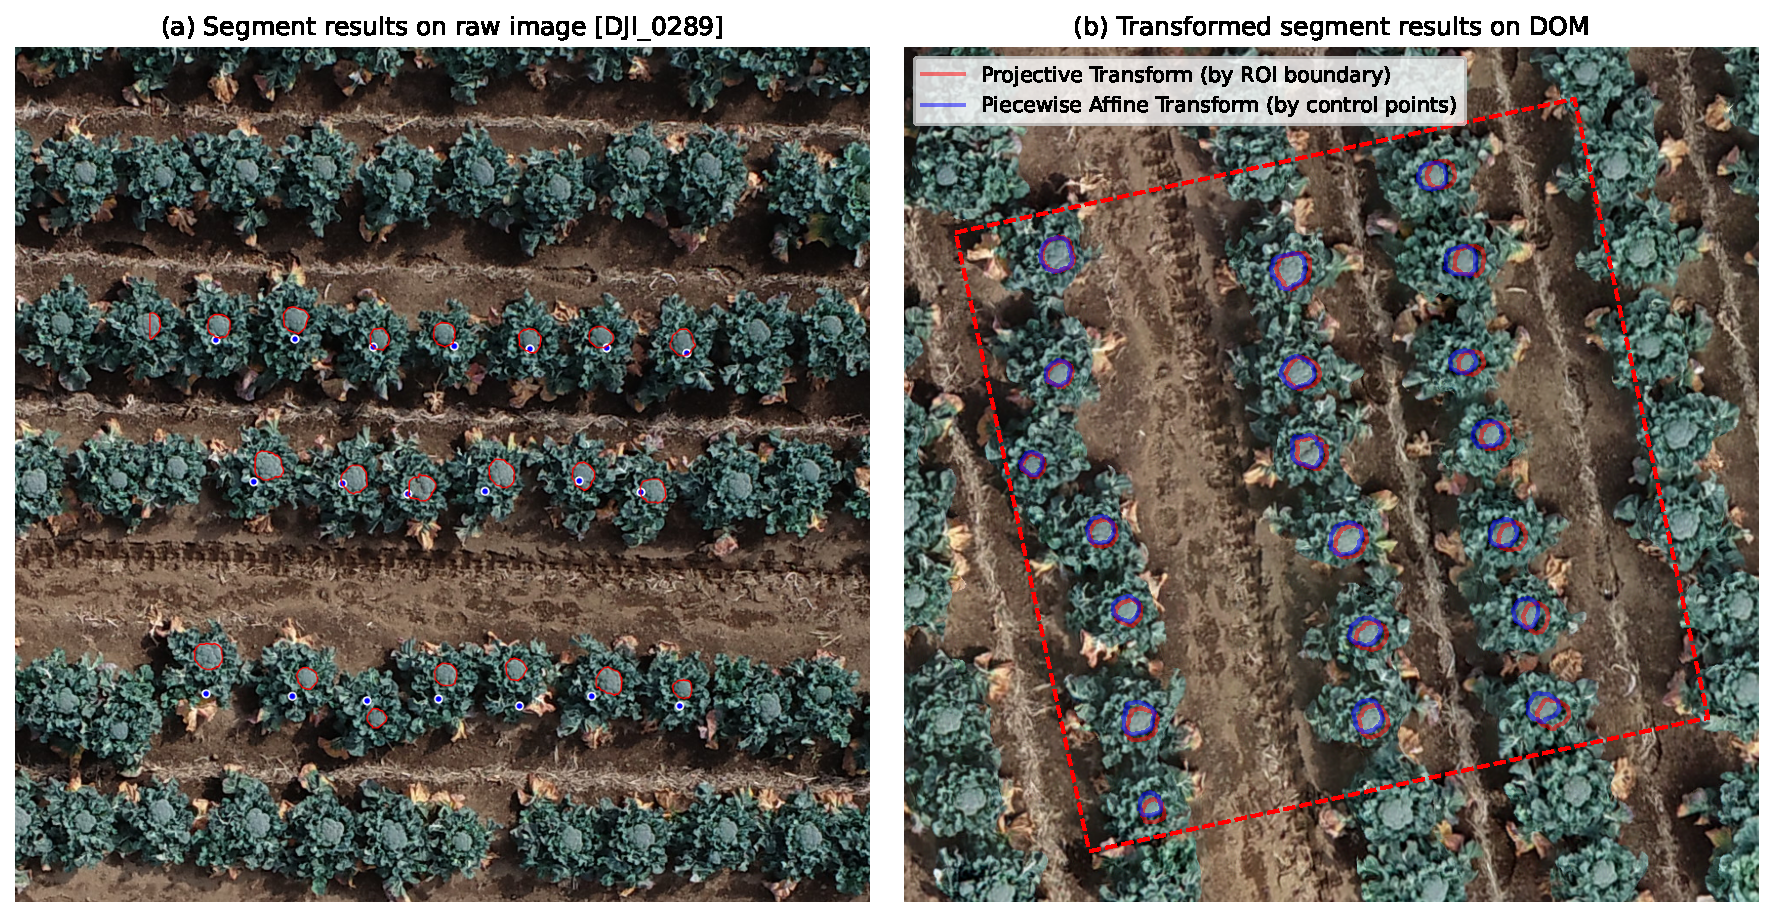
\includegraphics{figures/xrs/trans_compare_220331_114_DJI_0289.pdf}
    }
  \end{center}
  \caption[Head segmentation forward location comparison between projective and piecewise affine transformation]{
    Head segmentation forward location comparison between projective (in Chapter 3) and piecewise affine transformation (this chapter). (a) is the head segmentation results on the raw image. They are forward transformed to corresponding positions on the \gls{dom} using two different transformations.
  }
  \label{fig:xrs3}
\end{figure}

\begin{table}[htb]
  \caption{The components of AutoML calibration model}
  \label{tbl:xrs1}
  % \begin{adjustwidth}{-0.05\textwidth}{-0.05\textwidth}
    \begin{center}
      \begin{tabular}{cccc}
        \hline
        \textbf{model id} & \textbf{rank} & \textbf{ensemble weight} & \textbf{type}       \\ \hline
        72                & 1             & 0.22                     & random forest       \\
        55                & 2             & 0.08                     & random forest       \\
        2                 & 3             & 0.02                     & random forest       \\
        73                & 4             & 0.28                     & random forest       \\
        69                & 5             & 0.24                     & random forest       \\
        67                & 6             & 0.06                     & k nearest neighbors \\
        20                & 7             & 0.10                     & k nearest neighbors \\ \hline
        \end{tabular}
    \end{center}
  % \end{adjustwidth}
\end{table}

\begin{figure}[htb!]
  \begin{center}
    \resizebox{\textwidth}{!}{
      \includegraphics{figures/xrs/validation4automl.pdf}
    }
  \end{center}
  \caption[Validation for the AutoML calibration model]{
    Validation for the AutoML calibration model.
  }
  \label{fig:xrs4}
\end{figure}


\begin{figure}[htb!]
  \begin{center}
    \resizebox{\textwidth}{!}{
      \includegraphics{figures/xrs/aerial_matched_compare_220405_29.pdf}
    }
  \end{center}
  \caption[The closest matched broccoli head template 3D model]{
    The closest matched broccoli head template 3D model to each aerial segmentation results. Different colors represent different broccoli heads.
  }
  \label{fig:xrs5}
\end{figure}

\begin{figure}[htb!]
  \begin{center}
    \resizebox{\textwidth}{!}{
      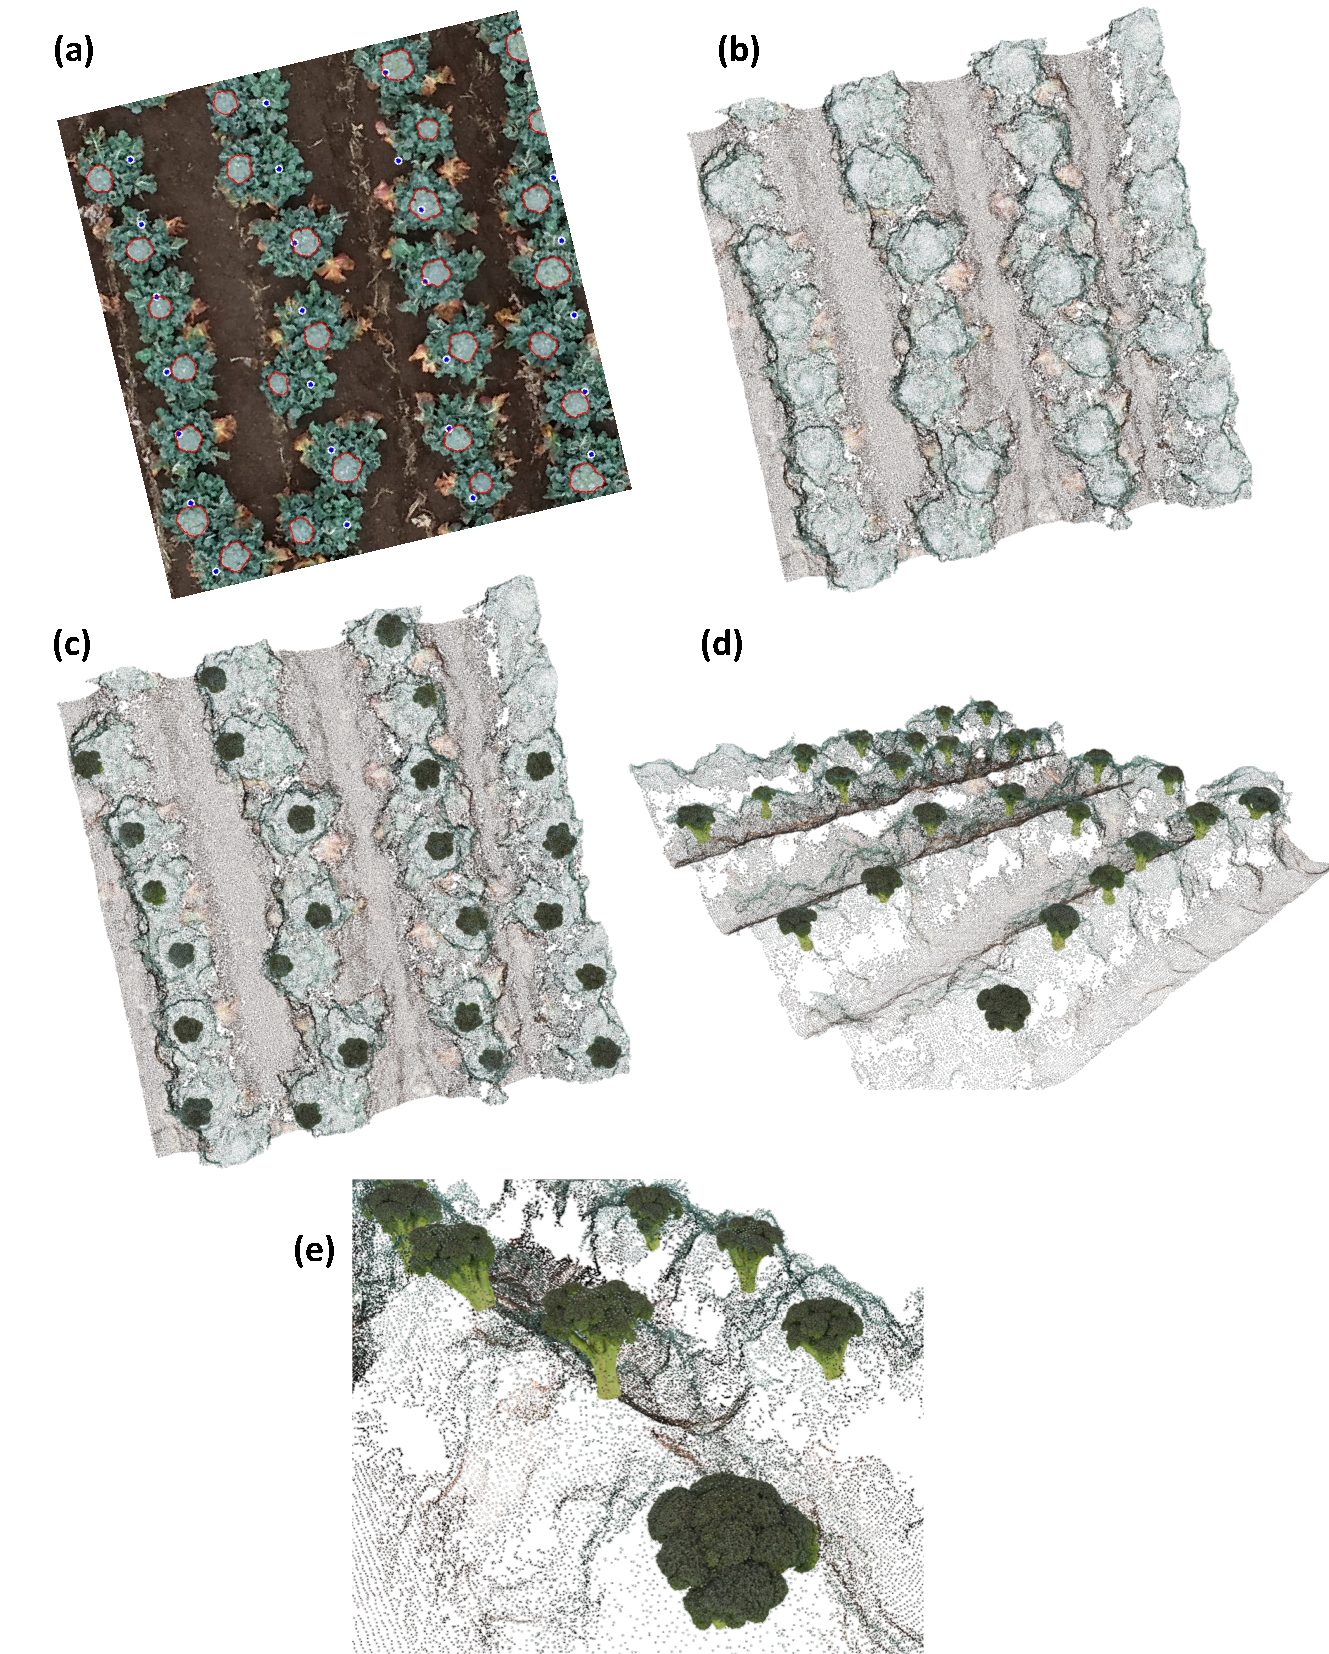
\includegraphics{figures/xrs/open3d_view.pdf}
    }
  \end{center}
  \caption[One example of 3D virtual visualization for optimal harvest date]{
    One example of 3D virtual visualization for optimal harvest date; (a) is the broccoli head segmentation results on raw aerial image; (b) is the top view of original aerial 3D point cloud models for broccoli canopy; (c) is the top view of canopy model with matched high-quality 3D broccoli heads; (d) is the side view; and (e) is the zoom in detailed view.
  }
  \label{fig:xrs6}
\end{figure}


\section{Discussion}

% 即使不进行校准(因为涉及到实际破坏性采样),

\section{Conclusion}